\chapter{The Physics of Gases}

The air you breathe is a blend of gases:
\begin{enumerate}
\item 78\% nitrogen in the form of $N_2$
\item 21\% oxygen in the form $O_2$
\item 1\% other gases (mostly argon)
\end{enumerate}

If you fill a balloon with helium ($He$),  the helium will push against the interior of the balloon with some pressure.   
The pressure is the same at every point in the interior of the balloon.  Pressure,  then,  is force spread over some area.   
Force is commonly measured in newtons.   Pressure is measured in \newterm{pascals}.  A pascal is 1 newton per square meter.

We don't usually think about it,  but the air outside the balloon is also pushing against the exterior of the balloon.  
We call this \newterm{barometric pressure} or \newterm{atmospheric pressure} and it is caused by gravity pulling on the gas molecules above the balloon.

\includegraphics[width=\textwidth]{balloon.png}


Imagine a square meter on the ground at sea level.  Now imagine the column of air above it -- reaching all the way to the top of the atmosphere.

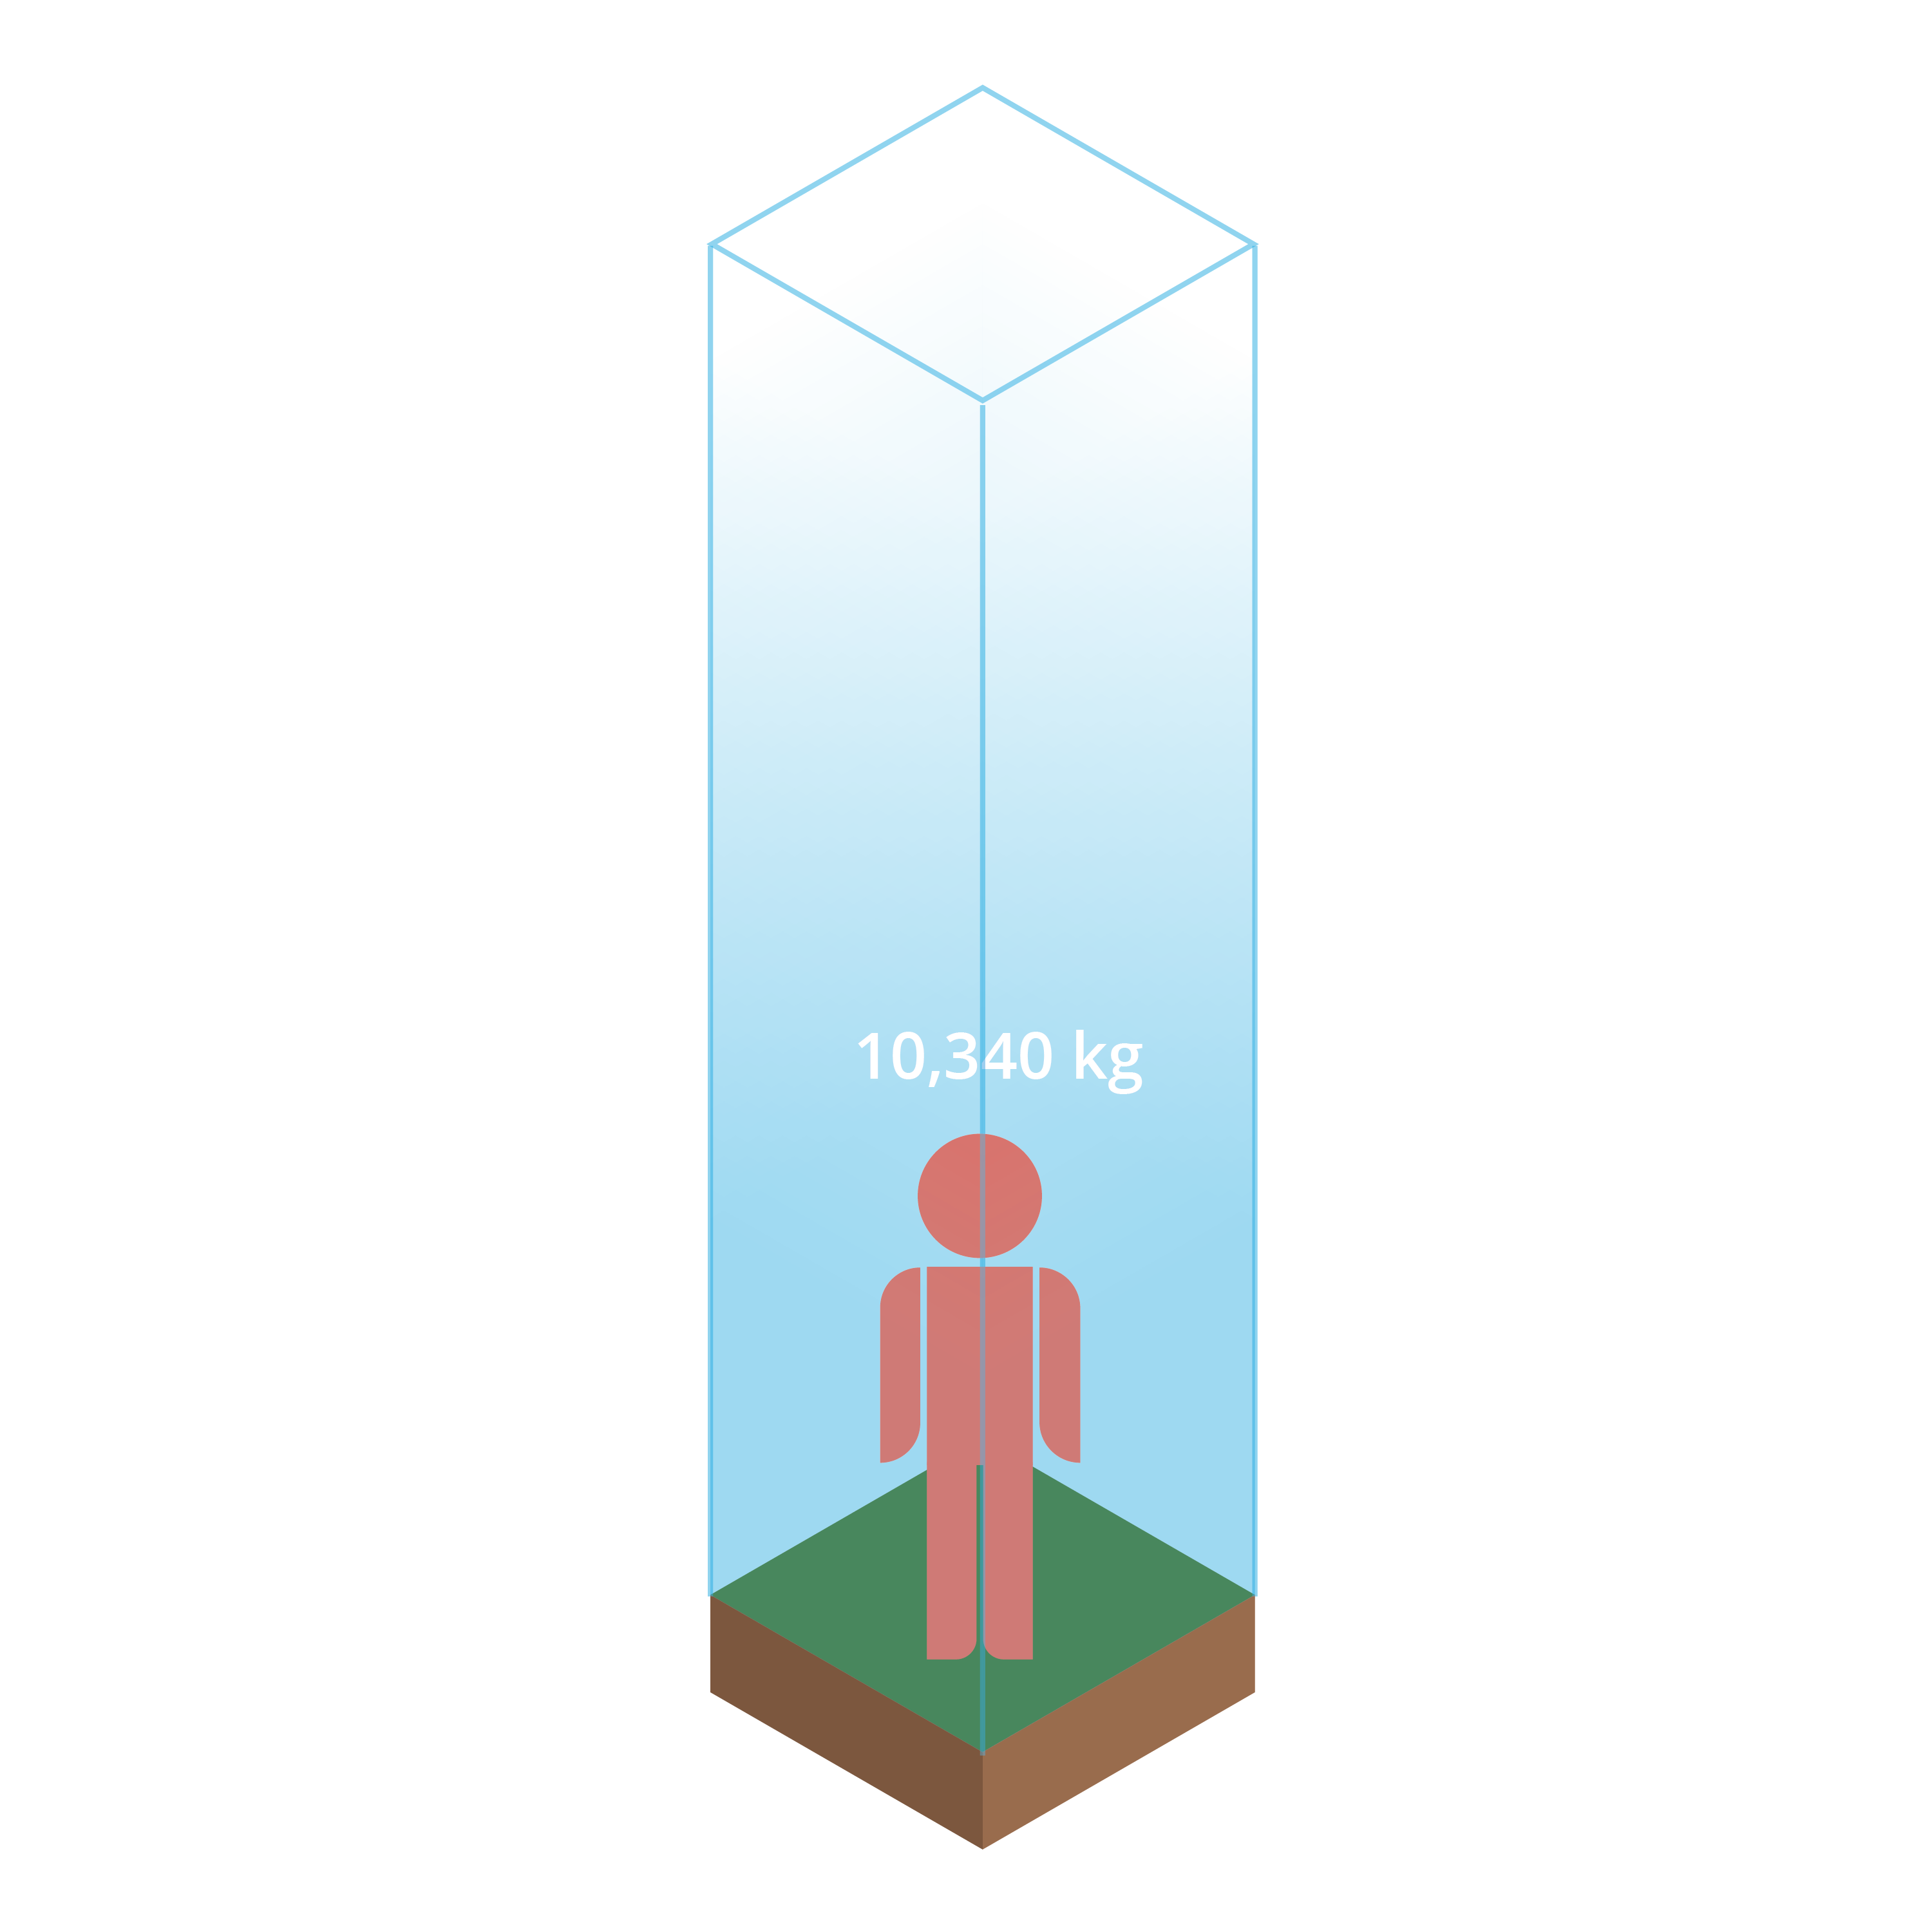
\includegraphics[width=\textwidth]{aircolumn.png}

The air inside that column has a mass of about 10,340 kg.  One kilogram on the earth experiences a gravitational force of 9.8 N.   
So the atmospheric pressure all around you is about 101,332 pascals.  
When dealing with such large numbers, we often use kilopascals.  
We'd say the barometric pressure at sea level is about 101.3 kPa.

That's a lot of pressure!  Why doesn't your ribcage collapse crushing your lungs?  The air \emph{inside} your lungs is the same 
pressure as the air push on the outside of your rib cage.  

And thus we live pretty much oblivious to this huge force that is all around us, but you can see it sometimes.  
For example, if you suck the air out of a plastic bottle,   the bottle will be crushed by the barometric pressure.

\section{Altitude and Atmospheric Pressure}

If you let go of the balloon, as it rises through this column there will be less and less air mass above it, and thus less and less atmospheric pressure on the outside of the balloon. 


\includegraphics[width=\textwidth]{balloonColumn.png}

What would be the atmospheric pressure at $h$ meters above sea level?  Here is a handy formula for that:

$$p = 101,332 \times \left(1 - \left( 2.25577 \times 10^{-5} \times h\right) \right)^{5.25588}$$

where $p$ is the atmospheric pressure in pascals.

\begin{Exercise}[title={Atmospheric Pressure},  label=atmos_pressure]
  
You are thinking about riding your bicycle to the top of Mount Everest.  You are worried when the atmospheric pressure outside the tire drops,  the tire will fail.  
(I have had a tire fail before; It is very, very loud.)  

Calculate the atmospheric pressure at the top of Mount Everest (9,144 meters above sea level).

\end{Exercise}
\begin{Answer}[ref=atmos_pressure]

$$p = 101,332 \times \left(1 - 2.25577 \times 10^{-5} \times h\right)^{5.25588}$$

and $h = 9,144$.  Thus,

$$p \approx 30.1 \text{kPa}$$

\end{Answer}

\section{The Temperature of a Gas}

Now,  let's say you start to heat the helium inside the balloon.  As the temperature goes up,  the molecules inside will start to move faster.

Remember that the kinetic energy of an object with mass $m$ and velocity $v$ is given by

$$k = \frac{1}{2} m v^2$$

So, you could say "As the temperature of the gas increases,  the kinetic energy of the molecules increases."   But a physicist would say "The temperature of the gas is how we measure its kinetic energy."

\subsection{A Statistical Look At Temperature}

If you say "This jar of argon gas is 25 degrees Celsius,"  you have told me about the \emph{average} kinetic energy of the molecules in the jar.  
However,  some molecules are moving very slowly.  Others are moving really,  really fast. 

We could plot the probability distribution of the speeds of the molecules.  For argon at 25 degrees Celsius,  it would look like this:

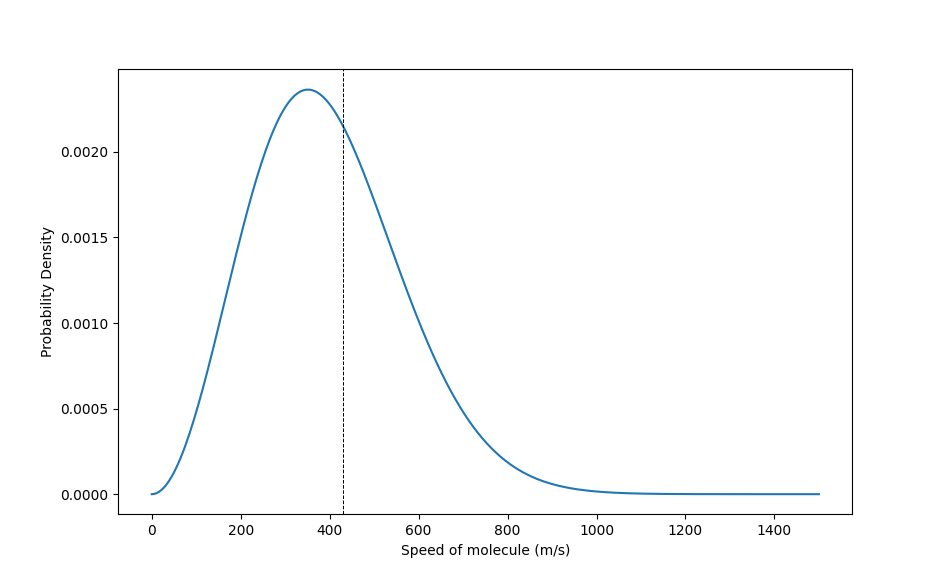
\includegraphics[width=\textwidth]{ar_plot.png}

The temperature,  remember,  is determined by the average kinetic energy of the molecules.  Some molecules are moving slowly and have less kinetic energy than the average.  Some molecules are moving very quickly and have more kinetic energy.  The dotted line is the divider between the two groups: molecules moving at speeds to the left of the line have less kinetic energy than average; those on the right have more kinetic energy than average.

Where is that line?  That is the RMS of the speeds of the molecules.  That is, if we measured all the speeds of all the molecules  $s_1, s_2, s_3, \ldots, s_n$, that line would be given by the root of the mean of the squares:

$$v_{rms} = \sqrt{\frac{1}{n} \left( s_1^2 + s_2^2 + s_3^2 + \ldots s_n^2 \right)}$$

If you have the same gas at a lower temperature, the distribution shifts toward zero:

Here is probability distribution of molecular speeds for argon gas at 25 degrees and -100 degrees Celsius.

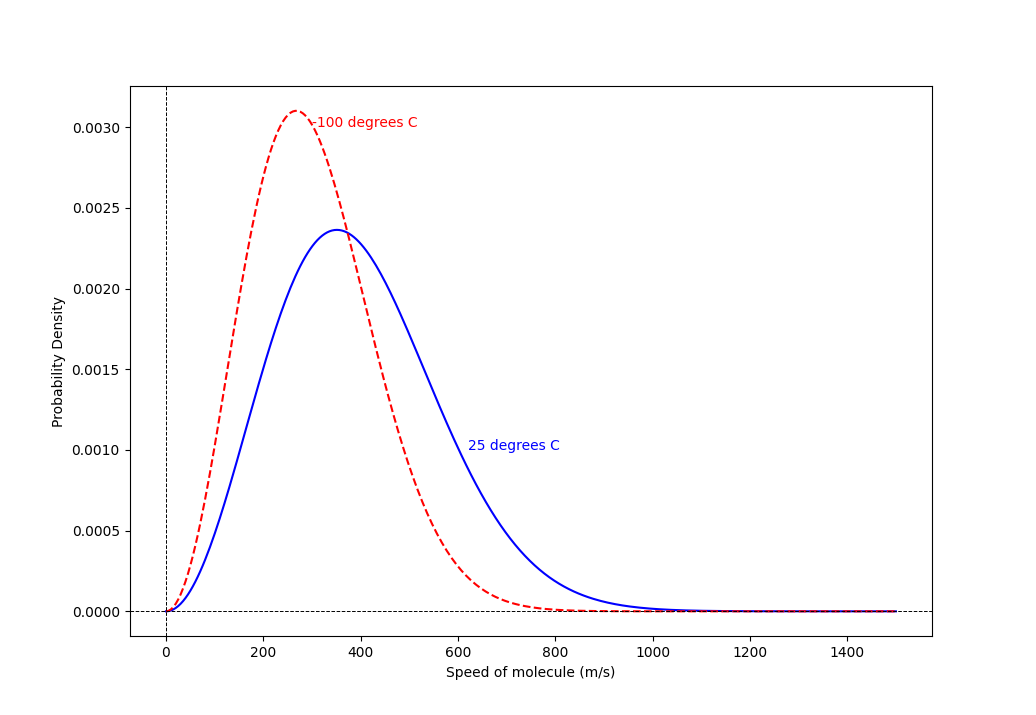
\includegraphics[width=\textwidth]{ar2_plot.png}

\subsection{Absolute Zero and Degrees Kelvin}

If you keep lowering the temperature,  eventually all the molecules stop moving.  This is known as \newterm{absolute zero} -- you
 can't make anything colder than absolute zero.   Absolute zero is -273.15 degrees Celsius.
 
Besides Celsius and Fahrenheit, there is a third temperature system: Kelvin.  The Kelvin has the same scale as Celsius, but it starts at absolute zero.   
So,  0 degrees Celsius is 273.15 degrees Kelvin.    And 100 degrees Celsius is 373.15 degrees Kelvin.

Any time you are working with the physics of temperature, you will use Kelvin.

Sometimes, when reading about gases, you will see "STP"  which stands for "Standard Temperature and Pressure."  STP is defined to be 100 kPa and $0^\circ$ Kelvin.

\section{Temperature and Volume}

Let's say you have a half-full air mattress in a field with a person lying on it around dawn.   The weight of the person will keep the pressure of the air inside constant (or pretty close).  

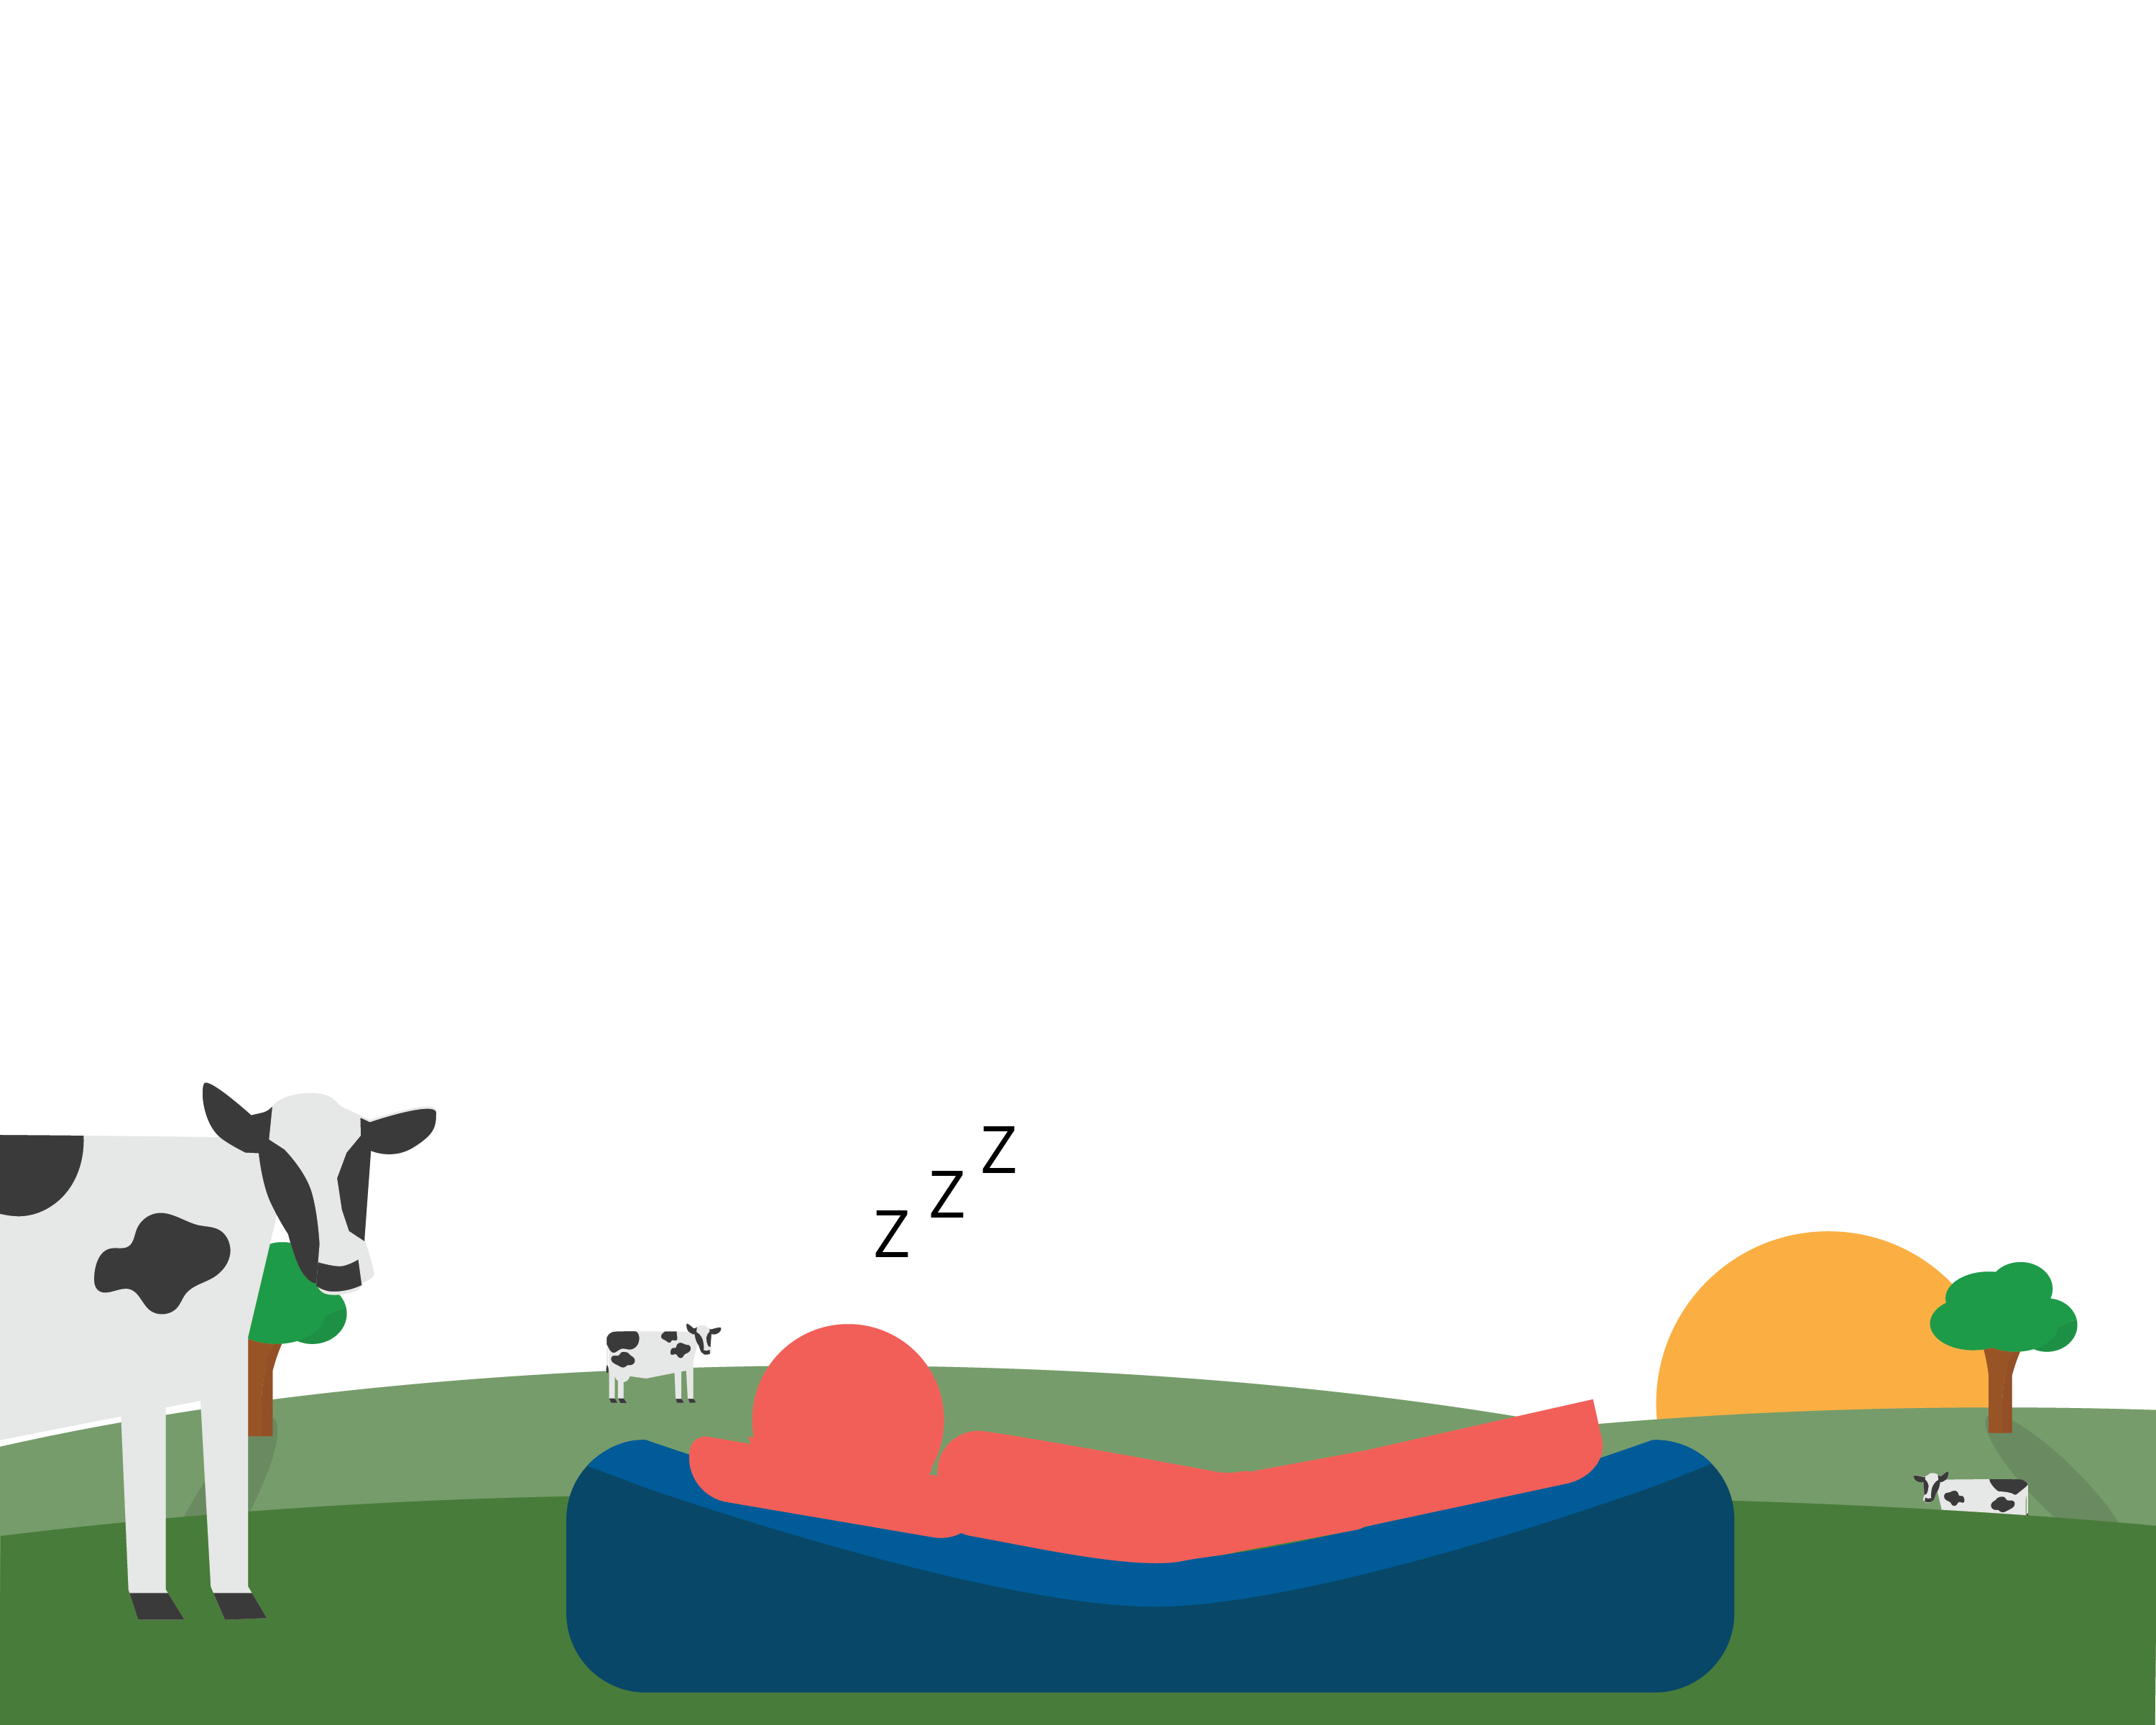
\includegraphics[width=\textwidth]{airMattress1.png}


The molecules in the mattress are not entering or leaving that mattress.  However, as the sun rises,  the air inside will get warmer and expand.  The person will be gently lifted by the expanding air.  You might wonder: how much will the air expand?


\includegraphics[width=\textwidth]{airMattress2.png}
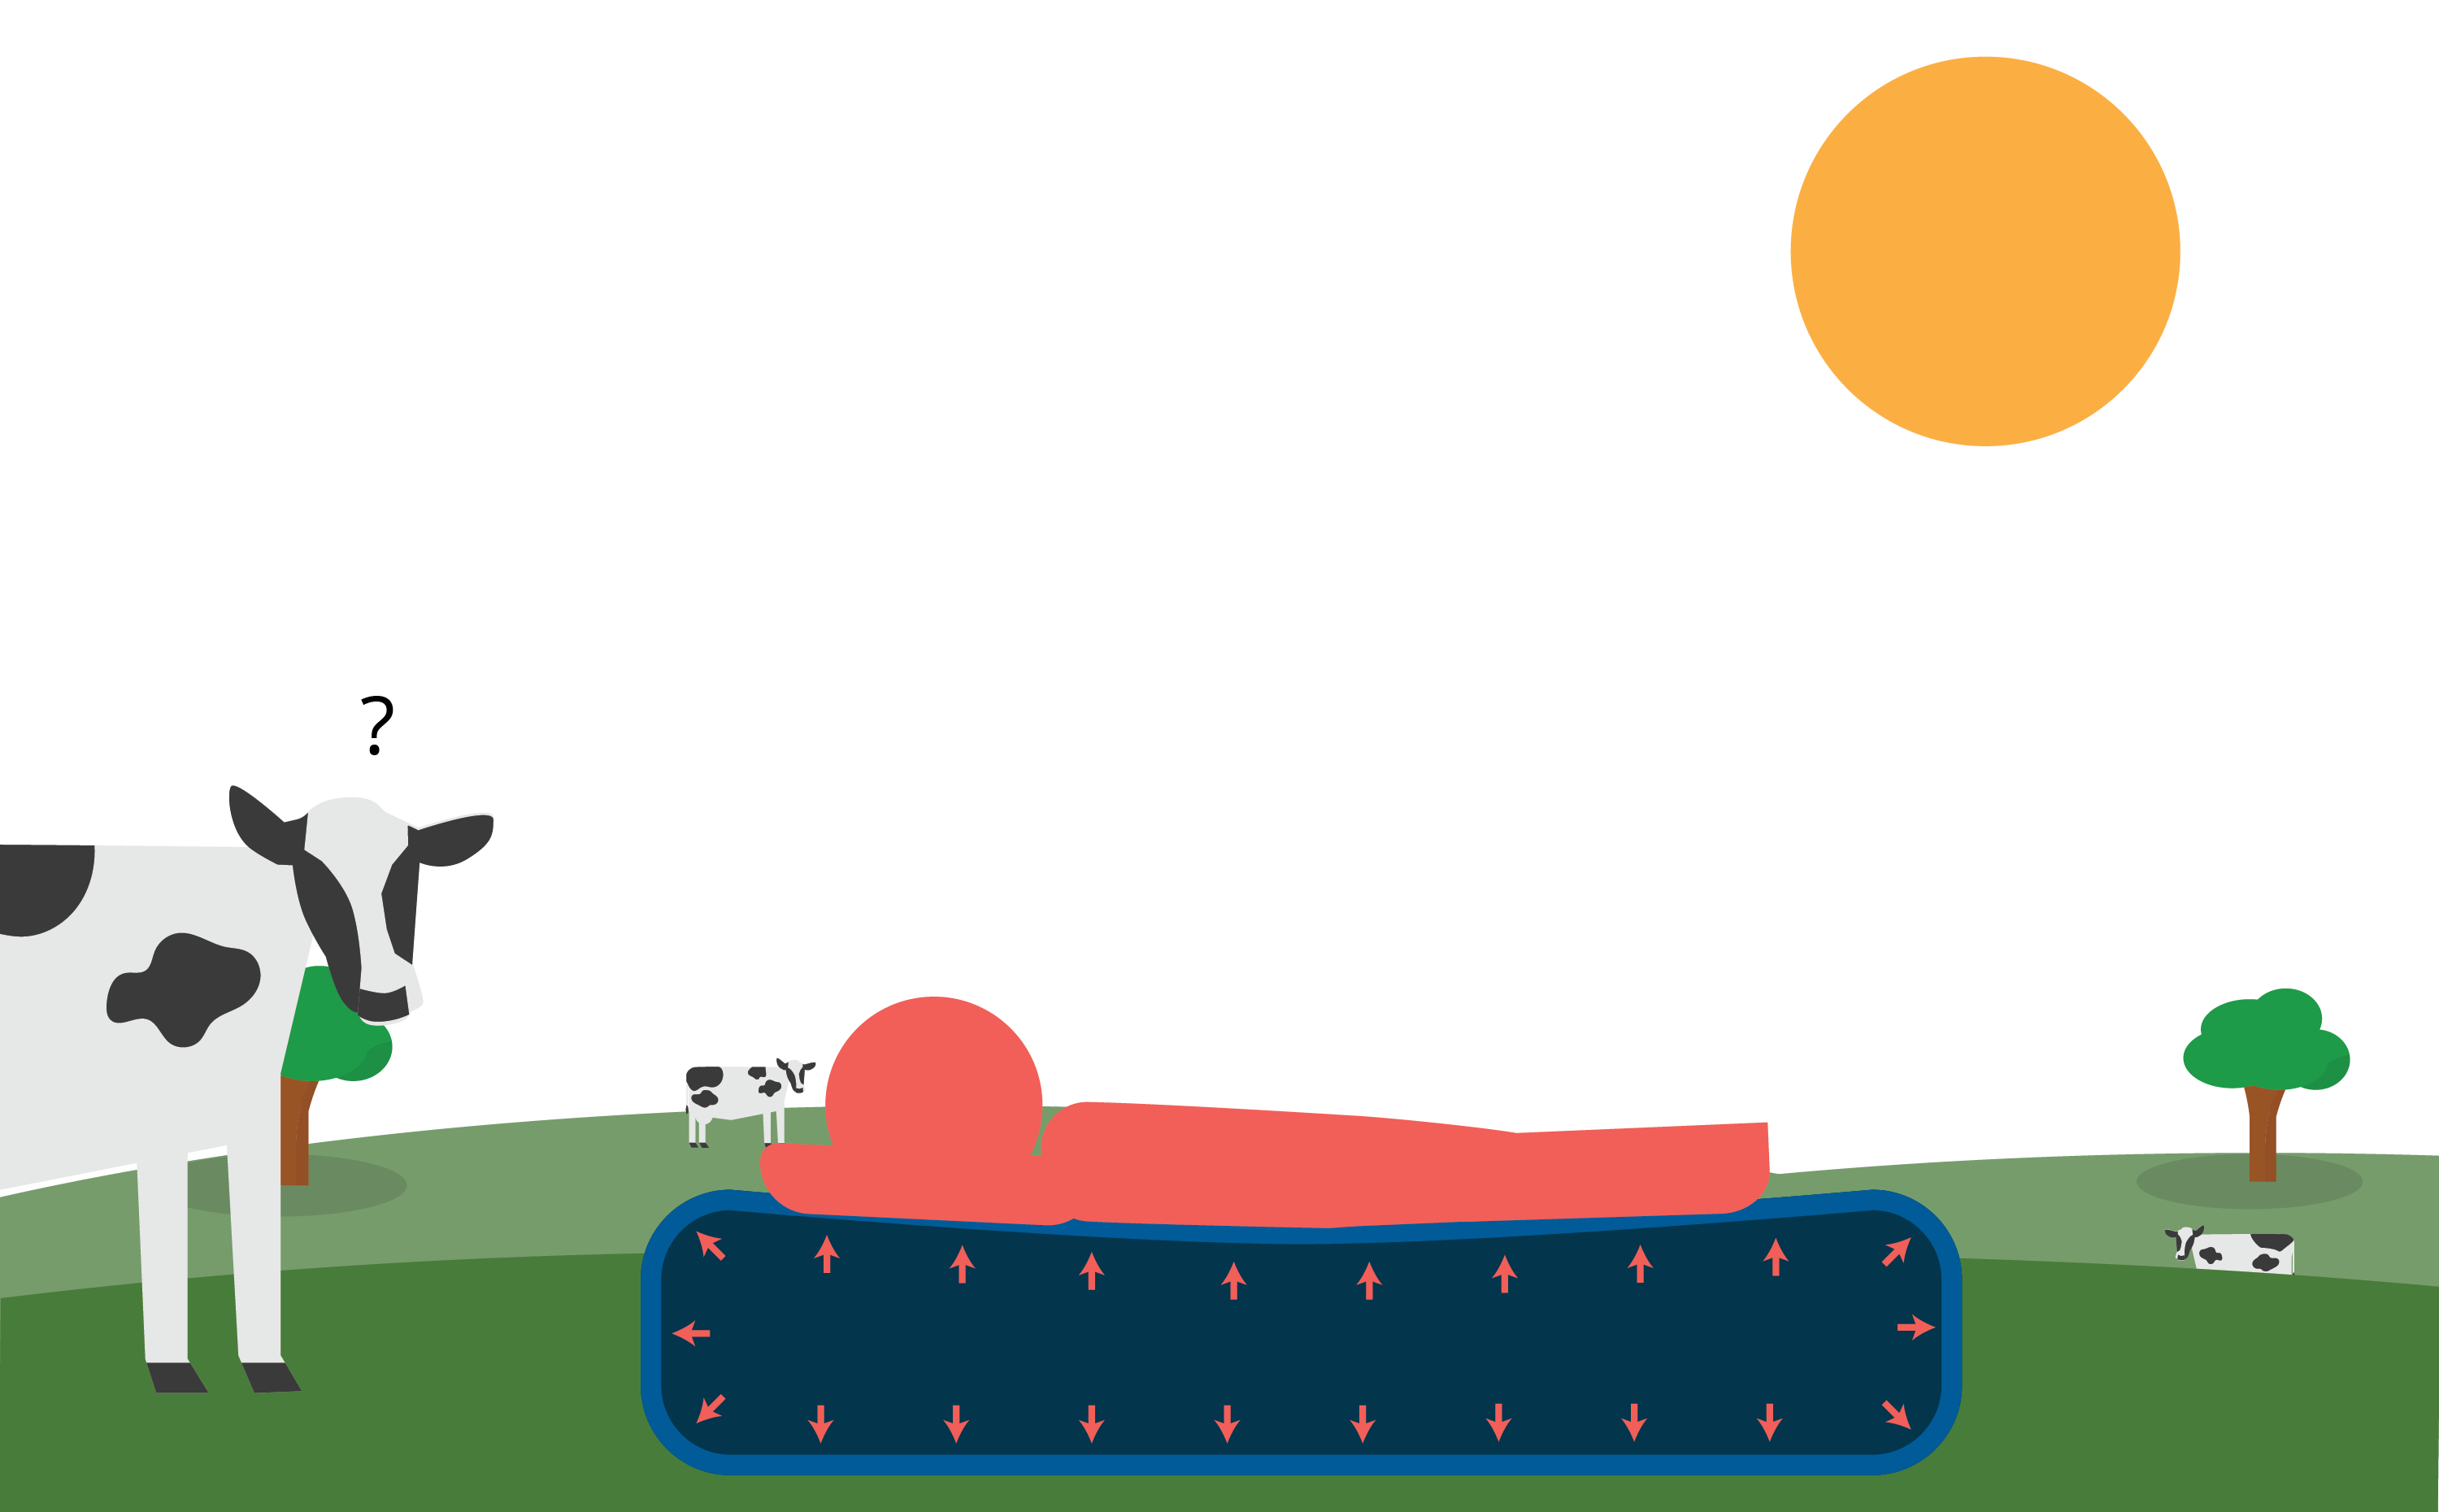
\includegraphics[width=\textwidth]{airMattress3.png}


If you have constant pressure and and a constant number of molecules,  the volume of the gas is proportional to the temperature in Kelvin:

$$V \propto T$$

\begin{Exercise}[title={Temperature and Volume},  label=temp_vol]
  
At dawn, the air inside mattress at dawn has a volume of 1000 liters and a temperature of 12 degrees Celsius.

At noon,  that same air has a temperature of 28 degrees Celsius.  The pressure on the gas has not changed at all.

What is the volume of the gas at noon?

\end{Exercise}
\begin{Answer}[ref=temp_vol]

First, we convert the temperatures into Kelvin:  
\begin{itemize}
\item Dawn: $12 + 273.15 = 285.15$
\item Noon: $28 + 273.15 = 301.15$
\end{itemize}

So, the temperature $T$ has increased by a factor of $\frac{301.15}{285.15} \approx 1.056$

Thus the volume of the air mattress has also increased by a factor of 1.056.  

So the air mattress that had a volume of 1000 liters at dawn,  will have a volume 1056 liters at noon.

\end{Answer}

Note: Volume and temperature are only proportional as long as the substance is a gas.   We will talk about liquids and solids soon.

\section{Pressure and Volume}

As you increase the pressure on a gas,  the molecules will get pushed closer together,  and the volume will decrease.

For example,  if you put the cap on an empty plastic bottle and squeeze it.   As you put the gas inside the bottle under pressure,  its volume will decrease. 

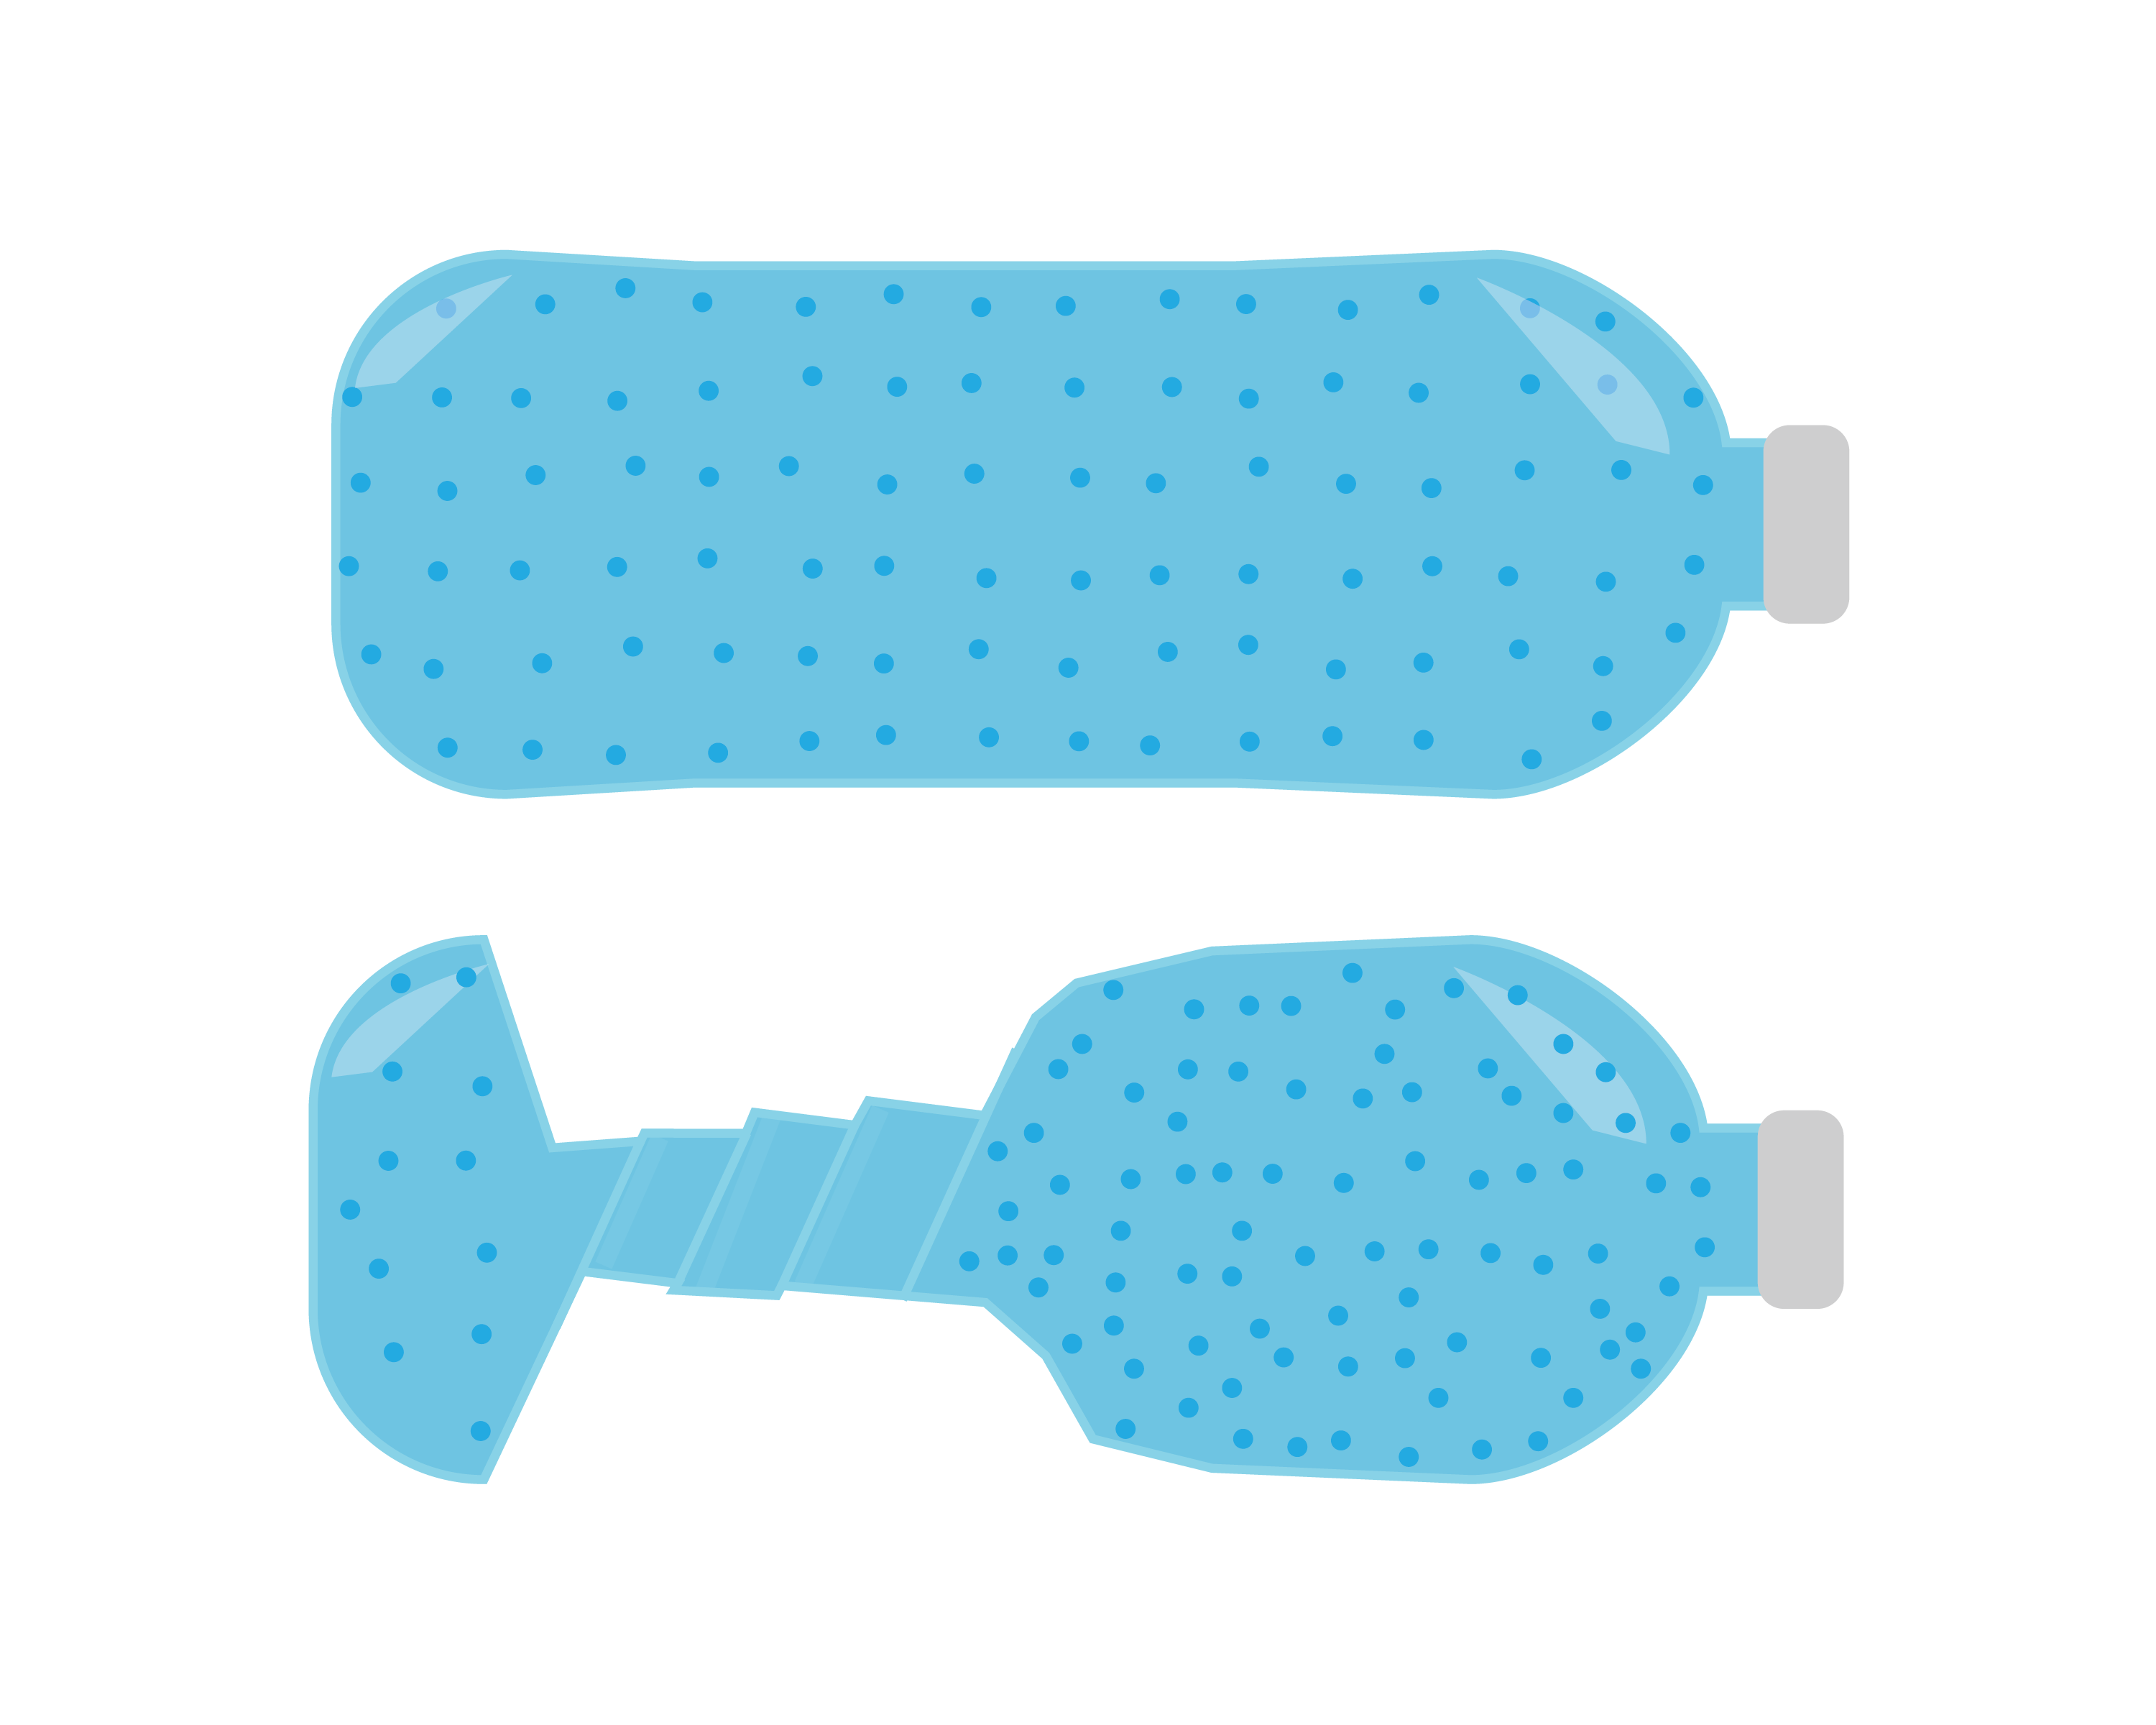
\includegraphics[width=\textwidth]{waterBottle.png}


If you keep the number of molecules and the temperature constant,  the pressure of the gas and its volume are inversely proportional:

$$P \propto \frac{1}{V}$$

"But," you say with disbelief, "if I increase the pressure on my empty water bottle from 5 kPa to 10 kPa,  the volume inside won't decrease by half!"

Don't forget that the air inside the bottle is under 101 kPa of atmospheric pressure before you even start to squeeze it.

\begin{Exercise}[title={Temperature and Volume},  label=temp_vol]
  
At an altitude where the atmospheric pressure is 100 kPa,  you seal air in a 1 liter water bottle.

Squeezing the water bottle,  you raise the internal pressure by 20 kPa  What is the volume inside the bottle now?

\end{Exercise}
\begin{Answer}[ref=temp_vol]

What is the pressure in kPA?  
\begin{itemize}
\item Before squeezing: 100 kPa
\item While squeezing: 120 kPa
\end{itemize}

So, the pressure $P$ has increased by a factor of $\frac{120}{100} = 1.2$

$1/1.2 \approx 0.833$

The air in the bottle had a volume of 1 liter before squeezing, so it has a volume of 833 milliliters while being squeezed.

\end{Answer}

\section{The Ideal Gas Law}

You are gradually getting an intuition for the relationship between the number of molecules, the volume, the pressure, and the temperature of a gas.
We can actually bring these together in one handy equation.

\begin{mdframed}[style=important, frametitle={Ideal Gas Law}]

$$PV = nRT$$

where:
\begin{itemize}
\item $P$ is the pressure in pascals
\item $V$ is the volume in cubic meters
\item $n$ is the number of molecules in moles
\item $R$ is the molar gas constant: 8.31446
\item $T$ is the temperature in Kelvin
\end{itemize}

(You can remember this as the "Pivnert.")

\end{mdframed}

From the name,  you might predict the following: The Idea Gas Law is not 100\% accurate.   But for most purposes,  it works remarkably well.  

Notice that the ideal gas law says nothing about what kind of gas it is; it works regardless.

\begin{Exercise}[title={Ideal Gas Law},  label=ideal_gas]
  
You have a cylinder containing $O_2$.  The chamber inside has a radius of 12 cm and a length of 50 cm.  
The temperature inside the cylinder is 20 degrees Celsius.
The pressure inside the tank is 600 kPa.

How many moles of $O_2$ are inside?

\end{Exercise}
\begin{Answer}[ref=ideal_gas]

First, let's convert the known values to the right unit:
\begin{itemize}
\item Radius = 0.12 m
\item Length = 0.5 m
\item $T = 20 + 273.15 = 293.15$ degrees Kelvin
\item $P = 600 \text{ kPa } = 600,000 \text{ Pa }$
\end{itemize}

The volume of the cylindrical chamber is $V = \pi r^2 h = \pi (0.12)^2 0 (0.5) \approx 0.0226$.

The Ideal Gas Law tell us that $PV = nRT$.  We are solving for $n$.

$$n = \frac{PV}{RT} = \frac{(600,000)(0.0226)}{(8.31446)(293.15)} \approx 5.68 \text{ moles of } O_2$$

\end{Answer}

\section{Molecules Like To Stay Close to Each Other}

When two molecules get close to each other a few things can happen:
\begin{itemize}  
\item They can under go a chemical reaction: electrons are exchanged or shared and a different molecule or molecules come into existence.  
This is the realm of chemistry, and we won't go into it in this course.
\item One or both of them have so much kinetic energy that they just pass each other or bounce off each other.  This is what happens in a gas.
\item The two molecules can "stick" together.  This is what happens in a liquid or a solid.
\end{itemize}

Why do they stick together if they aren't combined in a chemical reaction?

First, they don't get \emph{too close}.  If they get too close,  their electron clouds repel each other with a strong force.  
This is what happens in a gas when two molecules bounce off of each other.

But if the molecules are quite close to each other,  there are forces that will attract them toward each other.  
These intermoleculare forces are beyond the scope of this course, but they called Van der Waals forces and hydrogen bonds.   
The strength of these forces vary based on the two molecules involved. 

Which is why some of the matter around you is in gas form (molecules that don't stick together at the temperature and pressure you are living in because they have weak attractive forces) and some is non-gas 
(gangs of molecules with stronger attraction that makes them clump together as a liquid or a solid at that same temperature and pressure).

But.  What if we change the temperature and pressure,  we can change if and how the molecules clump together.  
This is known a \newterm{phase change}; We will cover it soon.